%!TEX root=main.tex
\subsubsection{Definiciones previas}
En base al estudio de los distintos diseños de alcuza disponibles en el mercado se clasificaron los diseños en 2 tipos principales: tradicional y no tradicional. Los cuales se definen a continuación.

\textbf{Tradicional:} Se entiende por un diseño tradicional aquel que está compuesto por botellas de vidrio o cerámica, de color transparente o monocromático con tapa de madera,  vidrio o metal. En adición puede poseer una bombilla adaptada.

\textbf{No tradicional:} Un diseño no tradicional será todo aquel diseño que no se clasifica como tradicional. De acuerdo a aquello esta variante posee alguna característica innovadora respecto del modelo clásico dominante. Entre ellas se pueden mencionar una adaptación diferente para aplicar el contenido, diseño en la pintura o forma  creativa.

En  cuanto a la definición del cliente final de las alcuzas, la investigación que se muestra en siguiente inciso permitió determinar dos tipos:

\textbf{Clientes tipo 1:} personas que compran una alcuza para su casa o para regalo.

\textbf{Clientes tipo 2:} restaurantes que compran alcuzas para su negocio.

\subsubsection{Demanda: Levantamiento de información}

En la actualidad el registro de datos públicos acerca de la demanda de alcuzas es nulo. No existe información detallada sobre la participación de mercado de cada una, ni sobre el volumen que ofertan las empresas que venden este producto. Por dicha razón, se utilizaron distintas metodologías para estimar los datos faltantes, en específico se realizaron entrevistas y encuestas, las cuales se detallan a continuación.

\begin{itemize}
\item \textbf{Entrevistas a tiendas comerciales:}
\end{itemize}

Las entrevistas se realizaron con los siguientes objetivos: conocer la cantidad de alcuzas vendidas al mes; identificar proveedores; averiguar qué diseños que tienen a la venta y sus respectivos ciclos de vida en la tienda; e indagar sobre las principales características de las personas que compran alcuzas.

Hasta el momento se han entrevistado 6 tiendas distintas, Paris, Falabella, Ripley, Casa\&Ideas, Kitchen Republic y Capdor. Cabe mencionar que la totalidad de las tiendas estaban ubicadas en el Mall Costanera Center.

En el Anexo \ref{PauEntRetail} se detalla la pauta de preguntas que se utilizó. Dicha guía está sujeta a flexibilidades, dado que cada entrevista se orientó según variaciones surgidas en el momento.

Las respuestas obtenidas permiten concluir que el perfil general de clientes que compran alcuzas es variado. Se identificaron los siguientes motivos de compra: adquisición para luego regalarla, realizar una reposición o al momento de mudarse a una casa nueva. En cuanto a tasa de ventas, se determinó que la tienda Falabella vende alrededor de 15 alcuzas al mes durante noviembre y diciembre, y el resto del año vende aprox. 5 alcuzas al mes. Las tiendas Kitchen Republic y Casa\&ideas venden 40 y 20 unidades mensuales, respectivamente.  La tienda Capdor vende entre 15 y 20 alcuzas al mes. En adición, según estimaciones de la vendedora entrevistada de Falabella, la proporción de ventas de alcuzas tradicionales y no tradicionales es 8:2. En el Anexo \ref{ResEntRetail} se muestra la información de forma detallada.

Durante las visitas a tiendas comerciales se investigaron las marcas o fábricas y los países de fabricación de las alcuzas. En el Anexo \ref{MarAlc} se muestra la lista obtenida.

\begin{itemize}
\item \textbf{Entrevistas a restaurantes:}
\end{itemize}

Las entrevistas se realizaron con el objetivo de conocer la cantidad de alcuzas que poseen los restaurantes en relación a la cantidad de mesas, determinar cuántas veces al año realizan reposición de alcuzas, averiguar cuales son sus proveedores de alcuzas y de aceite, obtener una aproximación del dinero que están dispuestos a pagar por una alcuza y, por último, percibir opiniones acerca del diseño que se está evaluando y conocer disposición a pagar por este.

En el Anexo \ref{PauEntRest} se detalla la pauta seguida en estas entrevistas, hasta el momento se han entrevistado 12 restaurantes, 10 ubicados en Providencia y 2 en Isla de Maipo. Los locales entrevistados fueron: Barandiara, Parrillada del Chef, Voraz, Sandwicheria \& Bistro, Diddlers Irish Bar \& Restaurant, Le Fournil, Luca’s, My Tavuk, Shopdog, Normandie, El Rincón Rústico y Ziufande.


Las entrevistas permitieron concluir que aquellos restaurantes que forman parte de una cadena o franquicia no compran alcuzas, sino que sus proveedores se las regalan o venden a un mejor precio. Por otro lado, la porción de restaurantes que si compran alcuzas prefiere diseños tradicionales  frente al diseño de alcuza integrada. Entre las razones que mencionaron fue que poseen un diseño de alcuza fijo en el local y realiza compra para reponer su \textit{stock} de alcuzas, y un diseño no tradicional implica educar al cliente acerca de su uso.

En cuanto a datos cuantitativos, se determinó que cada restaurante posee aproximadamente 1 alcuza por mesa y que se realiza reposición de alcuzas una vez al año. En el Anexo \ref{ResResEntRest} se muestra una tabla resumen de los Resultados de las entrevistas. En forma adicional, en el Anexo \ref{ResEntRest} se muestran las respuestas de cada restaurante de forma detallada.

\begin{itemize}
\item \textbf{Encuestas a personas:}
\end{itemize}

Los principales objetivos de la encuesta son: obtener una estimación de la demanda de alcuzas en general; indagar si las personas conocen el producto y lo utiliza en su casa a diario; determinar el perfil de los posibles compradores del producto; conocer su comportamiento de compra y preferencias; y averiguar la disposición a comprar el diseño de alcuza integrada.

Las encuestas se realizaron en el camino entre la estación de metro Tobalaba y el centro comercial Mall Costanera Center, entre las 15:00 y 18:30 hrs. durante un día domingo. Cabe destacar que el sondeo abarcó a 57 personas.  En el  Anexo \ref{PauEnc} se detallan las preguntas realizadas. Para la posterior utilización de los datos se supuso que cada persona entrevistada representó a un hogar, debido a que el producto estudiado está presente en forma unitaria en las casas, esta última información se corroboró al momento de realizar la encuesta.

Las encuestas permitieron determinar que el 57,9\% de los encuestados poseen una alcuza en su casa. El 35,1\% de las personas encuestadas utiliza a diario la alcuza al momento de comer. En cuanto al comportamiento de compra se concluyó que el 33,4\% compró una alcuza hace menos de 3 años y el 26,4\% compró una alcuza durante el año 2016. En el Anexo \ref{ResEncPer}  se muestran las respuestas tabuladas.


\begin{itemize}
\item \textbf{Entrevistas a empresas de aceite:}
\end{itemize}

Los objetivos de las entrevistas a empresas productoras de aceite son: indagar acerca de sus proveedores de envases de vidrio, conocer la cantidad de envases de vidrio que compra la empresa mensualmente, determinar si la organización es proveedor directa de restaurantes, averiguar si la empresa cuenta con el servicio de venta o regalo de alcuzas a sus clientes y conocer la forma en que producen o compran las alcuzas.

Las organizaciones entrevistadas fueron Las Doscientas y Olivos Ruta del Sol, la primera fue realizada presencialmente mientras que la segunda se realizó mediante correo electrónico. En el Anexo \ref{PauEntEmpAce} se muestra la pauta de preguntas realizadas.

De las dos empresas entrevistadas, una empresa es proveedora directa de aceite de oliva a restaurantes, además posee su propio diseño de alcuza, el cual  vende a cierta cantidad de restaurantes en forma exclusiva. En adición se averiguó que el proveedor de envases de vidrio de ambas empresas es Cristalerías Toro. En el Anexo \ref{ResEntEmpAce} se muestran las respuestas detalladas de las entrevistas.

Cabe destacar que las entrevistas y encuestas sirvieron como una primera aproximación al mercado, y en el futuro se espera realizar más indagaciones de la misma forma que aporten mayor solidez a los datos obtenidos.

\subsubsection{ Participación de mercado}

Para determinar la participación de mercado se realizó el cálculo del porcentaje de ventas que corresponde a alcuzas tradicionales, para ello se utilizaron los datos obtenidos en las entrevistas a tiendas comerciales. Aquello permitió determinar qué aprox. el 80\% de las alcuzas vendidas corresponden a alcuzas de diseño tradicional y el resto no tradicional (esto para el caso de los locales que venden ambos tipos de diseño).

Se utilizó la venta mensual de alcuzas obtenida mediante de las entrevistas a tiendas comerciales, luego este dato se amplificó por la cantidad de sucursales que posee dicha tienda en la Región Metropolitana. Con ello se obtuvo una venta escalada a la región. Luego se determinó la cantidad total de ventas de alcuza tradicional con la suma ponderada de las ventas de la región con el 80\% correspondiente a porcentaje de alcuzas tradicionales a la venta. La cantidad total de ventas de alcuza no tradicional se calculó de forma similar, pero esta vez se ponderó la venta total por 20\%, correspondiente a las ventas de alcuzas no tradicionales. La Tabla \ref{PartMercAlcu} muestra los datos utilizados y resultados obtenidos.

\begin{table}[H]
\centering
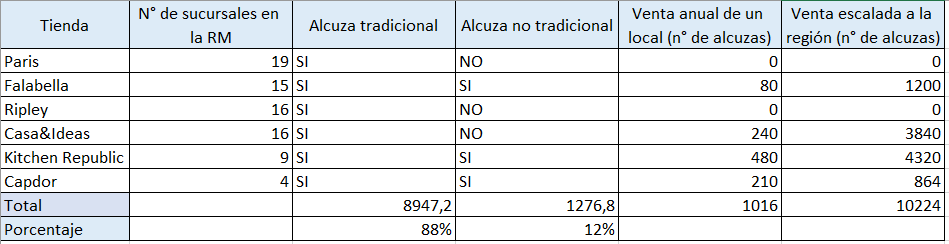
\includegraphics[width=\textwidth]{PartMercAlcu.png}
\caption{Participación de mercado de alcuzas, con datos obtenidos mediante entrevistas a tiendas.}
\label{PartMercAlcu}
\end{table}

Con los cálculos anteriores se determinó el porcentaje de ventas de alcuzas tradicionales el cual fue de 88\%, mientras que el porcentaje de venta de alcuzas no tradicionales es de 12\%.

Luego se utilizó la información disponibles de las páginas web de las principales tiendas  comerciales para determinar el promedio de alcuzas no tradicionales a la venta. Se estudió la gama de alcuzas que tienen a la venta las tiendas Falabella, Paris, Homy, Homecenter, Ripley, Casa\&Ideas, Easy, Morph, Kitchen Republic, Capdor, El Volcán, Imahe y Gangas. A partir de dicha información se determinó que el mercado, considerado en su totalidad, ofrece 48 diseños distintos de alcuzas tradicionales y 17 diseños de alcuzas no tradicionales. En el Anexo \ref{PartMerc} se encuentra la totalidad de datos tabulados.

Para estimar la participación del mercado que tendría la alcuza de sistema integrado se considera que esta debe ingresar al mercado y competir con las restantes alcuzas no tradicionales. Además, se supuso que no existe una preferencia significativa entre las distintas alcuzas no tradicionales, es decir, que la preferencia de los consumidores distribuye de forma uniforme entre los distintos tipos de diseños no tradicionales. Con todo lo anterior se concluye que la alcuza de sistema integrado utilizará 1/18  del mercado de alcuzas no tradicionales.

Por lo tanto el porcentaje que ocupará la alcuza integral dentro del mercado total del alcuzas será:

\begin{equation*}
\text{Porcentaje de participación de alcuza integrada} = 0.12 \times 100 \times \frac{1}{18} = 0.17\%
\end{equation*}

\subsubsection{Estimación de la demanda en la Región Metropolitana}

Las entrevistas realizadas a tiendas de retail permitieron determinar un periodo de 3 años para realizar el estudio. Además esto  se respalda por Estadísticas del Servicio de Impuestos Interno, las cuales afirman que la vida útil de enseres de vidrio de hoteles y restaurant tiene una duración de 3 años. \footnote{
Información disponible en \url{http://www.sii.cl/pagina/valores/bienes/tabla_vida_enero.htm} )
}
Para estimar la demanda, se consideraron por separado los dos tipos de cliente.
\paragraph{Demanda de Clientes tipo 1}

Para estudiar la demanda de clientes tipo 1 se propusieron dos metodologías, las cuales se detallan a continuación.

\textbf{Metodología 1:}  En base a información de encuestas a personas.

Para comenzar se realizará una estimación de la cantidad de hogares que existen en la RM.  Para ello se obtuvo un estimado de la población de la región y la cantidad de personas promedio por hogar, como se detalla a continuación.


Se obtuvo la población de los años 2017 a 2020 en las proyecciones del INE a partir del CENSO del año 2002  \cite{ine1}.

Se determinó el número de personas por hogar  según el CENSO del año 2002, el cual indica que en la Región Metropolitana este número es aproximadamente 3,75 \cite{ine2}. Se asumirá que este número es constante.

Con lo anterior se determinó la cantidad de hogares con la siguiente expresión:

\begin{equation*}
\mbox{N}^o\text{ de hogares} = \frac{\text{población en la Región Metropolitana}}{\text{Cantidad de personas por hogar}}
\end{equation*}

Luego, a partir, de la encuesta realizada se obtuvo la demanda anual con la pregunta n$^o$ 10 (ver Anexo \ref{PauEnc} y \ref{ResEncPer}). En ella se obtuvo el porcentaje de hogares que compró una alcuza durante el año 2016, con lo cual se obtuvo una estimación de la demanda anual de alcuzas. Dado que la cantidad de alcuzas que compraron durante el año 2016 fue de 16, equivalente al 28\% del total de personas encuestadas. En base a dichos datos se calculó la cantidad de hogares que compraría una alcuza en un año de la siguiente forma:


\begin{equation*}
\mbox{N}^o\mbox{ de hogares que compran} = \mbox{N}^o\mbox{ de hogares}\times 0,28
\end{equation*}

La expresión anterior representa la demanda total del alcuzas en un año.

Luego la cantidad de hogares que compran la alcuza integrada se determinará utilizando el porcentaje de participación del mercado determinada anteriormente (0,7\%). Los cálculos se muestran a continuación:

\begin{equation*}
\mbox{N}^o\mbox{ de hogares que compran alcuza integrada} = \mbox{N}^o\mbox{ de hogares que compran}\times 0,007
\end{equation*}

\textbf{Metodología 2:  Ciclo de vida del producto}

Dado el carácter de innovación del SAI se consideró que el Modelo de Bass era propicio para estudiar el ciclo de vida del producto.

La expresión matemática del modelo discreto es la siguiente:
\begin{equation*}
S_t=(P+Q(\frac{Y_{t-1}}{M}))(M-Y_{t-1}).
\end{equation*}
Donde $P_t$ es la citada probabilidad, $Y_{t-1} $ en número de compradores servidos hasta $t$ (o número de compradores acumulados en $t-1$) y $P$, $Q$ y $M$ son parámetros. Dado que $Y_0=0$, se cumple que $P_1=P$, es decir, $P$ es el parámetro que recoge el impacto inicial de la innovación, ya que determina la probabilidad de compra cuando todavía no existen usuarios previos; se denomina tasa de innovación. El parámetro $M$ expresa la población de potenciales usuarios del producto y se supone constante. Por lo tanto, $\frac{Y_{t-1}}{M}$ es la fracción de saturación del mercado en el período $t$. El parámetro $Q$ refleja el impacto de los usuarios previos sobre la probabilidad de compra y se denomina tasa de imitación o de difusión.


Referencias bibliográficas \cite{aleman2007estrategias} indican que el valor medio de $P$ está en torno a 0,02; mientras que el valor de $Q$ oscila entre 0,4 y 0,5. Por ello los parámetros utilizados para los cálculos fueron $P=0.02$ y $Q=0.45$ . El parámetro $M$ fue determinado como la cantidad de población que no posee una alcuza en su casa, esto se calculó con el porcentaje de personas que poseen alcuza en su casa (57.9\%, dato obtenido de la encuesta realizada), la predicción de la población de la región para los próximos 3 años y la probabilidad de comprar una alcuza (28\%,dato obtenido de la encuesta realizada). A continuación, se muestra la expresión para calcular el parámetro $M$.

\begin{equation*}
M=0,579\times 0,28 \times \mbox{Población de la región predicha para dicho año}
\end{equation*}

\paragraph{Demandas de clientes tipo 2}

Para el segundo tipo de clientes, los restaurantes, se puede comentar lo siguiente. Respecto a ellos las entrevistas señalaron que, en general, los restaurantes que cuentan con más de un local compran las alcuzas directamente a sus proveedores de aceites o estos últimos se los regalan por motivos de marketing. De la totalidad de restaurantes entrevistados que caen en esta categoría, sólo uno se mostró dispuesto a cambiar el producto tradicional por otro basado en el diseño que se está evaluando, sin embargo, señaló que solo lo compraría si el producto es más barato que el utilizado actualmente. Es por esta razón, que con los datos actuales que se tienen se concluyó que esta clase de restaurantes no adquirían este nuevo diseño de alcuza.

Los restaurantes más pequeños entrevistados compran las alcuzas al por mayor. Dos de ellos señalaron que podrían cambiar al diseño que se está evaluando, pero se mostraron reticentes a ello. Se cree que puede existir un tipo de restaurante que esté más interesado en este diseño, pero no se tienen datos de ello, por lo que solo se utiliza la demanda obtenida del primer tipo de cliente por el momento.

\subsubsection{Escalamiento de la demanda a Chile}

Para escalar los datos de la demanda hacia todo Chile se utilizó información acerca de la predicción de la población por cada región del país. Se obtuvo la población de los años 2017 a 2020 en las proyecciones del INE a partir del CENSO del año 2002.

Los cálculos para ambos casos fueron realizados de forma análoga a los mostrados en los incisos anteriores, a diferencia de que la predicción de la población de cada región fue propia de cada sitio.

En las tablas \ref{DemandaChileMet1} y \ref{DemandaChileMet2} se muestran los resultados obtenidos con las Metodologías 1 y 2 correspondientemente. En ellas se puede observar que mediante la Metodología 1 se estimó un total de 28.168 unidades de SAI demandadas, mientras que la Metodología 2 indicó un total de 49.718 unidades.

\begin{figure}[H]
\centering
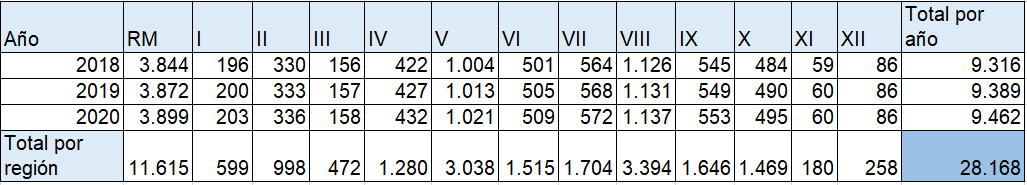
\includegraphics[width=\textwidth]{DemandaChileMet1.png}
\caption{Demanda en Chile, metodología 1.}
\label{DemandaChileMet1}
\end{figure}

\begin{figure}[H]
\centering
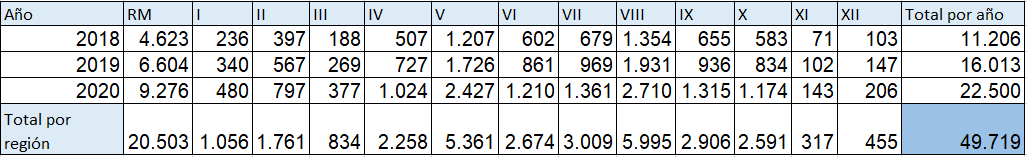
\includegraphics[width=\textwidth]{DemandaChileMet2.png}
\caption{Demanda en Chile, metodología 2.}
\label{DemandaChileMet2}
\end{figure}

\subsubsection{Precios de mercado}

Para determinar el precio de mercado de la alcuza integrada primero se obtiene el precio de venta de las alcuzas no tradicionales en las tiendas de retail. Luego, se estima el costo en adquirir dichas alcuzas a las tiendas. Dicho costo corresponde al precio al cual la empresa productora de alcuzas le vende el producto a las tiendas. A continuación se detalla el cálculo de cada paso.

En primer lugar se obtuvieron los precios de mercado de las alcuzas no tradicionales, esto se realizó a en base a catálogos de internet.  A partir de aquí se decide el precio al que se vendería la alcuza en el retail.

\begin{figure}[H]
\centering
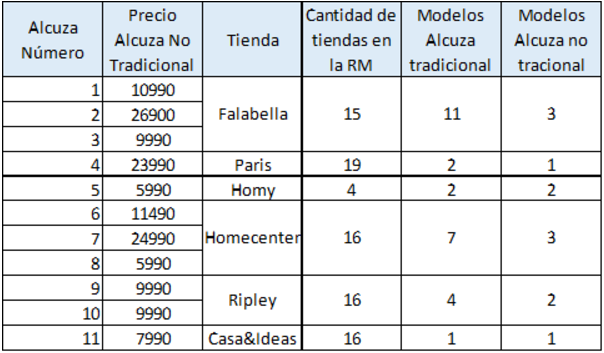
\includegraphics[scale=1.]{Precios.png}
\caption{Precios de las alcuzas no tradicionales.}
\label{Precios}
\end{figure}

Para determinar el precio al cual se venderá la alcuza, sin disponer de mayor información acerca del mercado y sus cuotas de distribución que los precios en las distintas tiendas, se plantea un problema básico de optimización de la cuota de mercado que se pretende alcanzar:
\begin{equation*}
\min \sum(P_i-P)^2
\end{equation*}

Donde $P_i$ es el precio de una alcuza no tradicional y $P$ es el precio al cual se venderá la alcuza integrada en el mercado. Tomando los datos de la Tabla \ref{Precios} el precio que maximiza la Cuota de Mercado Óptima (CMO) es \$14.175. La distribución de los precios y el óptimo se ve reflejada en la Figura \ref{GraficoPrecio}.

\begin{figure}[H]
\centering
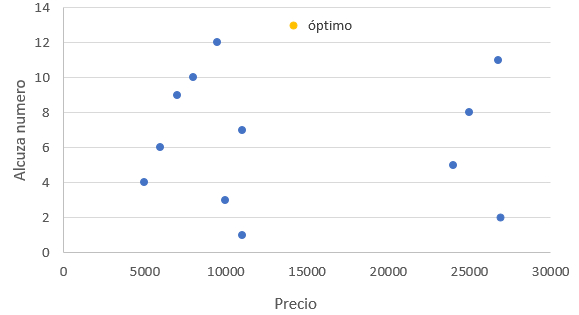
\includegraphics[scale=1.]{GraficoPrecio.png}
\caption{Determinación Cuota Mercado Óptima.}
\label{GraficoPrecio}
\end{figure}

Sin embargo, el modelo planteado debe implementar ciertas restricciones que se deben añadir al modelo una vez que se disponga de mayor información del mercado y además asume ciertos supuestos:
\begin{itemize}
\item Consumidores son racionales, demanda uniforme
\item Competencia no ajusta sus precios
\item Se debe considerar la elasticidad-precio de la demanda
\end{itemize}


En segundo lugar se determinó el porcentaje de costo sobre ingresos. Para este cálculo se utilizó el estado financiero de la tienda Fababella 2016 \cite{falabella}. En ella se muestra un de actividades ordinaria de 7.898.301.784 y un costo de ventas de 5.180.719.944, con lo que se obtiene que el costo de venta es el 66\% del ingreso por actividades ordinarias. Por lo tanto, el 66\% del precio óptimo de venta en retail es
\$$14.175 \times 0.66=\$9.355$, es decir, el precio de mercado de la alcuza integrada será de \$$9.355$.

Para obtener un costo más representativo se quiere seguir indagando en las empresas de retail, esto para obtener un margen promedio.

\subsubsection{Volumen a ofertar}

El volumen a ofertar del negocio que se está evaluando es el máximo entre el pedido mínimo que se puede mandar a hacer y la demanda estimada. Esto debido a que si no se hace el pedido mínimo se fabricarían 0 alcuzas, lo que sería equivalente a no producir, por lo que se tiene que producir al menos eso; y porque conviene producir a la demanda estimada si esta es mayor que el pedido mínimo.

Por un lado, se realizó una cotización a Cristalchile por el pedido mínimo que acepta, el cual es de 50.000. Por otro lado, la demanda total de alcuzas estimada mediante las 2 metodologías fue de 28.168 y 49.718 unidades, por lo que el volumen a ofertar será de 50.000 unidades.
